\documentclass[10pt,letterpaper]{article}
\usepackage[top=1in,bottom=1in,left=1in,right=1in]{geometry}
\usepackage{datetime}
\usepackage{natbib}      % http://merkel.zoneo.net/Latex/natbib.php
\usepackage{palatino}
\usepackage{verbatim}
\usepackage[normalem]{ulem}
\bibpunct{(}{)}{;}{a}{,}{,}

\usepackage{array}

\usepackage{chngpage}
\usepackage{stmaryrd}
\usepackage{amssymb}
\usepackage{amsmath}
\usepackage{graphicx}
\usepackage{lscape}
\usepackage{subfigure}
\usepackage[usenames,dvipsnames]{color}
\definecolor{myblue}{rgb}{0,0.1,0.6}
\definecolor{mygreen}{rgb}{0,0.3,0.1}
\usepackage[colorlinks=true,linkcolor=black,citecolor=mygreen,urlcolor=myblue]{hyperref}

\newcommand{\bocomment}[1]{\textcolor{Bittersweet}{BO says: #1}}

\newcommand{\inner}[1]{\langle #1 \rangle} 
\newcommand{\smallsec}[1]{\noindent \textbf{#1\ }}
\newcommand{\cmd}[1] {{\color{blue}\texttt{#1}}}

\newcommand{\solution}[1]{{\color{myblue} \emph{[Solution:} 

#1 

\emph{End solution]}}}
\newcommand{\solutionnote}[1]{{\color{myblue} \emph{[Note:}

#1 

\emph{End note]}}}
\newcommand{\points}[1]{{\color{mygreen}\emph{[#1]\ \ }}}

\newcommand{\aone}{\diamondsuit}
\newcommand{\atwo}{\heartsuit}
\newcommand{\bone}{\triangle}
\newcommand{\btwo}{\Box}
\newcommand{\myand}{\ \land\ }
\newcommand{\myor}{\ \lor\ }
\newcommand{\mynot}{\lnot}

\title{
  \textbf{Mini-project 2} \\
  \Large{CMPSCI 670, Fall 2019, UMass Amherst} \\
  \Large{Instructor: Subhransu Maji} \\
  \Large{TAs: Aruni Roy Chowdhury, Archan Ray}
}

\settimeformat{ampmtime}
\date{}
\begin{document}
\maketitle

\renewcommand\thesubsection{\thesection.\alph{subsection}}


\section*{Guidelines}

\paragraph{Submission.} Submit a \emph{single pdf document} via Gradescope that includes your solutions, figures and code. The latex source file for the homework is provided which you can modify to produce your report. You are welcome to use other typesetting software as long as the final output is a pdf. For readability you may attach the code printouts at the end of the solutions within the same pdf. Note that we will not run your code. Similarly figures should be included in a manner which makes it easy to compare various approaches. Poorly written or formatted reports will make it harder for the TA to evaluate it and may lead to a deduction of credit. 

\paragraph{Late policy.} You could have 24 hours late submission with a 50\% mark down. Late submission beyond 24 hours will not be given \emph{any} credits. 

\paragraph{Plagiarism.} We might reuse problem set questions from previous years, covered by papers and webpages, we expect the students not to copy, refer to, or look at the solutions in preparing their answers. We expect students to want to learn and not google for answers. See the Universities' guidelines on academic honesty (\url{https://www.umass.edu/honesty}).

\paragraph{Collaboration.} The homework must be done individually, except where otherwise noted in the assignments. 'Individually' means each student must hand in their own answers, and each student must write their own code in the programming part of the assignment. It is acceptable, however, for students to collaborate in figuring out answers and helping each other solve the problems. We will be assuming that you will be taking the responsibility to make sure you personally understand the solution to any work arising from such a collaboration. 

\paragraph{Using other programming languages.} We made the starter code available in Python and Matlab. You are free to use other languages such as C, Java, Octave or Julia with the caveat that we won't be able to answer or debug language-questions.

\paragraph{Python requirements.} We will be using Python 2.7. The Python starter code requires \cmd{scipy}, \cmd{numpy} (at least v1.12), and \cmd{scikit-image}.
If you are not familiar with installing those libraries through some package manager (like \cmd{pip}), the easiest way of using them is installing \href{https://conda.io/docs/user-guide/install/index.html}{Anaconda}.\\


\newpage
\section{Color image demosaicing [30 points]}
Recall that in digital cameras the red, blue, and green sensors are interlaced in the Bayer pattern (Figure~\ref{fig:bayer}). The missing values are interpolated to obtain a full color image. In this part you will implement several interpolation algorithms. 



Your entry point for this part of the homework is in \cmd{evalDemosaicing}. The code loads images from the data directory (in $\cmd{data/demosaic}$), artificially mosaics them (\cmd{mosaicImage} file), and provides them as input to the demosaicing algorithm (\cmd{demosaicImage} file). The input to the algorithm is a single image im, a NxM array of numbers between 0 and 1. These are measurements in the format shown in Figure~\ref{fig:bayer}, i.e., top left \cmd{im(1,1)|im[0,0]} is red, \cmd{im(1,2)|im[0,1]} is green, \cmd{im(2,1)|im[1,0]} is green, \cmd{im(2,2)|im[1,1]} is blue, etc. Your goal is to create a single color image C from these measurements.
\begin{figure}[h]
\centering
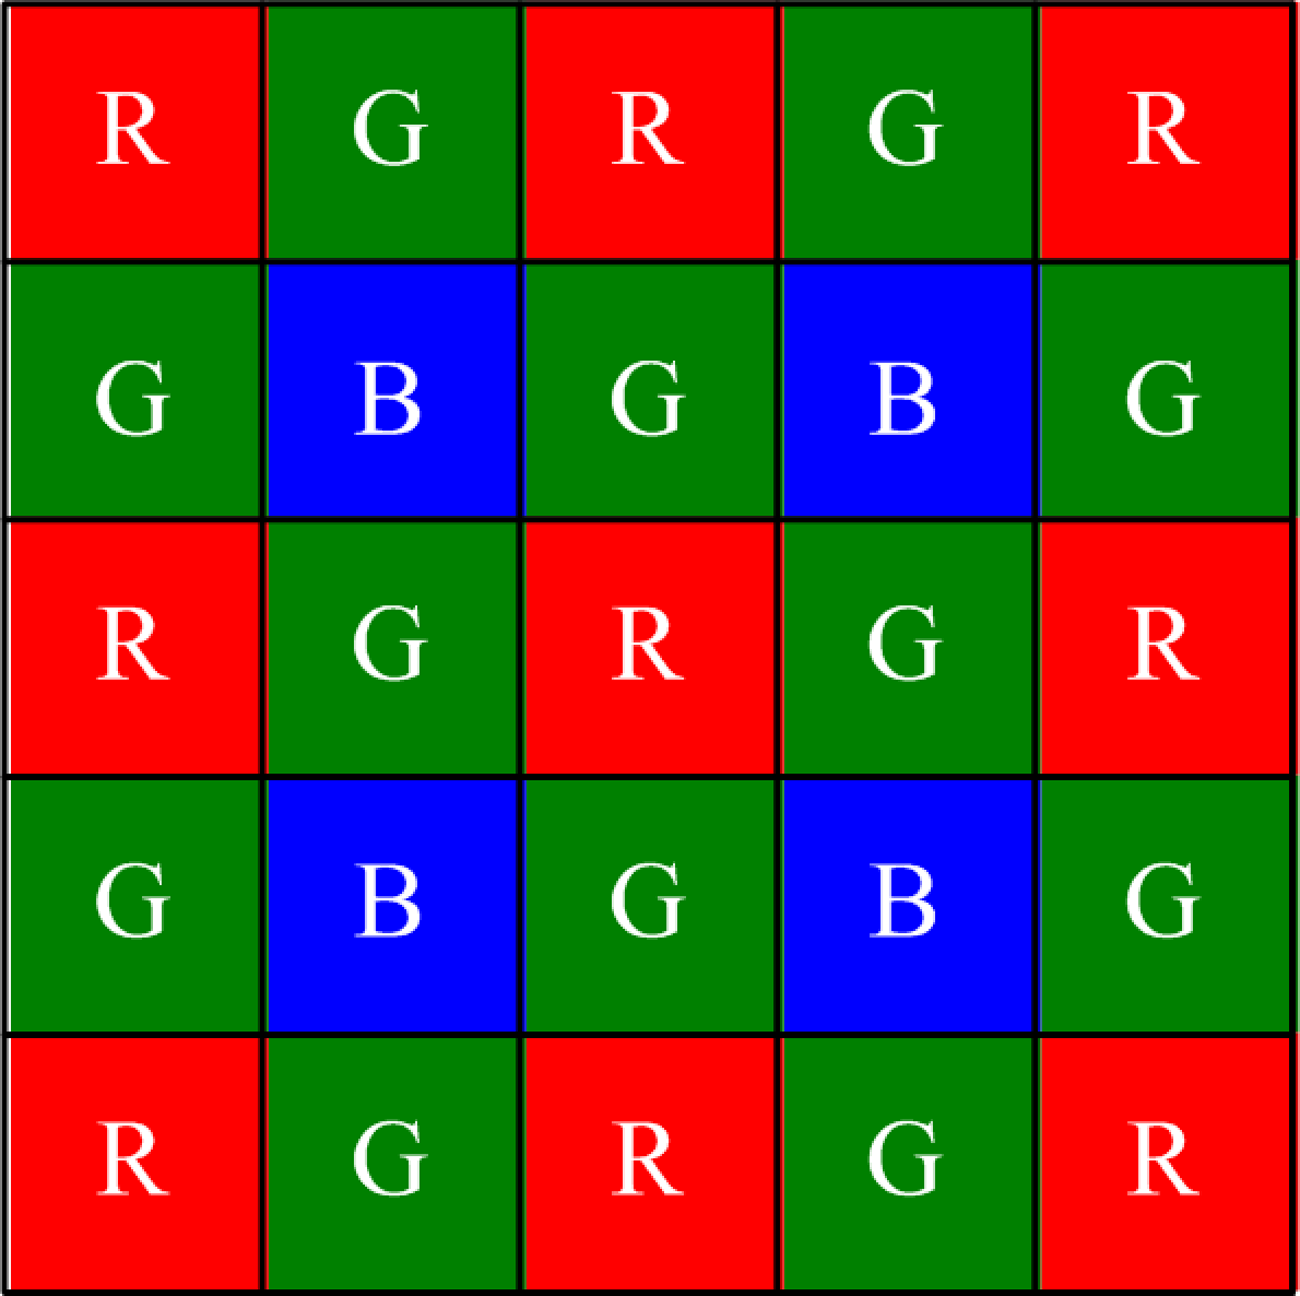
\includegraphics[width=0.2\linewidth]{bayer-pattern.png}
\caption{\label{fig:bayer} Bayer pattern}
\end{figure}

By comparing the result with the input we can also compute the error measured as the distance between the estimated image and the true image. This is what the algorithm reports. Running \cmd{evalDemosaic} from the Matlab command prompt produces the output shown below:

\begin{verbatim}
----------------------------------------------------------------------------
#    image             baseline      nn       linear     adagrad
----------------------------------------------------------------------------
1    balloon.jpeg      0.179239    0.179239    0.179239    0.179239 
2    cat.jpg           0.099966    0.099966    0.099966    0.099966 
3    ip.jpg            0.231587    0.231587    0.231587    0.231587 
4    puppy.jpg         0.094093    0.231587    0.231587    0.231587 
5    squirrel.jpg      0.121964    0.231587    0.231587    0.231587 
6    pencils.jpg       0.183101    0.183101    0.183101    0.183101 
7    house.png         0.117667    0.117667   0.117667   0.117667 
8    light.png         0.097868    0.097868    0.097868    0.097868 
9    sails.png         0.074946    0.074946    0.074946    0.074946 
10  tree.jpeg         0.167812   0.167812    0.167812    0.167812 
----------------------------------------------------------------------------
    average             0.136824   0.136824    0.136824    0.136824 
----------------------------------------------------------------------------
\end{verbatim}

Right now only the \cmd{demosaicImage(im, 'baseline')} is implemented which simply replaces all the missing values for a channel with the average value of that channel (while using python codes, if you're getting any warnings regarding \textbf{iCCP}, do \cmd{mogrify *.png} in the \cmd{data/demosiac} folder). All the other methods call the baseline algorithm and hence they produce identical results. Implement the following functions in the file:

\begin{itemize}
\item \textbf{[10 points]} \cmd{demosaicImage(im, 'nn')} -- nearest-neighbour interpolation.
\item \textbf{[10 points]} \cmd{demosaicImage(im, 'linear')} -- linear interpolation.
\item \textbf{[10 points]} \cmd{demosaicImage(im, 'adagrad')} -- adaptive gradient interpolation.
\end{itemize}

In class we discussed how to interpolate the green channel. For the red and blue channels the algorithms will be different since there are half as many pixels with sampled values. For the adaptive gradient method start by interpolating only the green channel and using linear interpolation for the other two channels. Once the overall performance is better, think of a way of improving the interpolation for the red and blue channels. You can even apply different strategies to different pixels for the same channel! 

For reference, the baseline method achieves an average error of 0.1392 across the 10 images in the dataset. Your methods you should be able to achieve substantially better results. The linear interpolation method achieves an error of about 0.017. To get full credit for this part you have to 
\begin{itemize}
\item include your implementation of \cmd{demosaicImage}, 
\item include the output of \cmd{evalDemosaic} in a table format shown earlier,
\item clearly describe the implementation details.
\end{itemize}

Tip: You can visualize at the errors by setting the display flag to true in the \cmd{runDemosaicing}. Avoid loops for speed in MATLAB/Python. Be careful in handling the boundary of the images.

\section{Depth from disparity [35 points]}

In this part of the homework, you will use a pair of images to compute a depth image of the scene.
You will do this by computing a disparity map.
A disparity map is an image that stores the displacement that leads every pixel in an image $X$ to its
corresponding pixel in the image $X^\prime$.
The depth image is inversely proportional to the disparity, as illustrated in Figure \ref{fig:disparity}.

\begin{figure}[h]
\centering
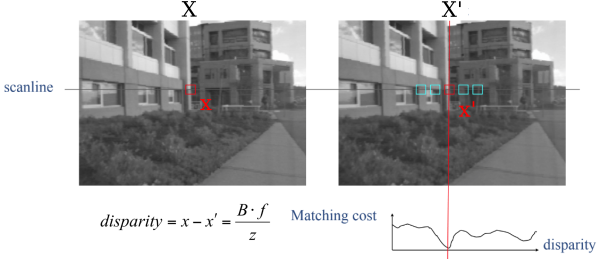
\includegraphics[width=0.7\linewidth]{fig/disparity.png}
\caption{\label{fig:disparity} Visual description of depth map computation from a pair of images.}
\end{figure}

In order to compute the disparity map, you will have to associate each pixel $x$ in $X$ with the corresponding
pixel $x^\prime$ in $X^\prime$.
This association can be computed by finding the image patch centered in $x^\prime$ that that has the smallest SSD
to the patch centered in $x$.
However, it is not necessary to compute SSD for every patch in $X^\prime$:
for this homework, you can assume that the images planes are parallel to each other and have the same focal length,
which means that you only need to search for the patches computed along the same epipolar line,
as illustrated in Figure \ref{fig:disparity}.

\begin{enumerate}
\item \textbf{[20 points] Compute depth image.}
For this part, you will implement the function \cmd{depthFromStereo}.
This function receives two images of the same scene and a patch size for SSD computation.
It returns an image containing the relative depth.
You can assume that the images planes are parallel to each other and have the same focal length.
Once you compute the disparity image by finding patch correspondences along the same epipolar line,
you can compute the depth through the following equation:
\begin{equation}
x-x^\prime = \frac{B f}{\text{depth}}
\end{equation}
where $B$ is the baseline and $f$ is the focal length. Notice that we don't have access to $B$ and $f$ values,
but those are constant throughout both images.
This means that you will not be able to compute the true depth image,
just the relative depth.

The entry code for this part is \cmd{evalDisparity}. The code loads a pair of images and you will implement a function that estimates the depth of each pixel in the first image, which you can visualize as a grayscale image. Assume $Bf = 1$ in your calculation. Show results for both pair of images included in the data directory. 

To get good results you might have to experiment with the window size and the choice of patch similarity measure. Try a few different ones and report what worked well for you. Include a short discussion of on what parts of the image does the approach work well and where it fails.

\item \textbf{[5 points] Discussion.}
In the first mini-project you implemented a method for depth estimation using photometric stereo.
Discuss advantages and disadvantages of stereo over photometric stereo.

\item \textbf{[10 points] Informative patches}. 
  Not all regions are equally informative
  for matching. 
  As we discussed in class, one way to measure how informative a patch
  is using its second-moment matrix. For a pixel $(u,v)$ this is
  defined as:
\begin{equation}
M = \begin{bmatrix}
             \sum_{x,y} I_{x}I_x            &  \sum_{x,y}I_{x}I_{y}\\
            \sum_{x,y}I_{x}I_{y}  &  \sum_{x,y}I_{y}I_y
        \end{bmatrix}, 
\end{equation}
  where the summation is over all pixels $(x,y)$ within a window around
  $(u,v)$. 
  $I_x$ and $I_y$ are the gradients of the image and can be computed
  using pixel differences, e.g., $I_x(u,v) = I(u+1, v) -
  I(u,v)$ and $I_y(u,v) = I_y(u,v+1) - I(u,v)$.
  The eigenvalues of $M$ indicate if the window is uniform, an
  edge, or a corner.

  Let $\lambda_1$ and $\lambda_2$ be the eigenvalues of the matrix
  $M$. 
  Write a function to compute the quantity $R = \lambda_1\lambda_2 - k(\lambda_1 +
  \lambda_2)^2$ for $k=0.03$ for each pixel given an image and window radius $r$. 
  Visualize this quantity for the images \cmd{tsukuba\_im1} and
  \cmd{poster\_im2} for radius $r = 5$ and $r=10$ as a heatmap (or
  grayscale image).
  What does the heatmap indicate? Describe this qualitatively.

  Include your implementation in the submission (call the method \cmd{visualizeInformation}.)
  You may find the following identities useful for calculating
  $R$. Given a $2\times 2$ matrix $M = [a~b; c~d]$, the $det(M) = \lambda_1
  \lambda_2 = ad-bc$ and $trace(M) = \lambda_1 + \lambda_2 = a + d$.

%  for this part would is \cmd{evalSecondOrderStats}. You are required
%  to edit the file \cmd{computeImageHeatmap} for solving this part of
%  the homework. The window size has already been set to 5 in file
%  \cmd{evalSecondOrderStats}.

%\begin{enumerate}
%    \item \textbf{Compute local patch moments}. For each image in the the directory  \cmd{../data/disparity}, compute the second moment matrix defined by: 
    
%    $M(u,v) = \sum_{(x,y) \in W} \begin{bmatrix}
%            I_{x}^2(u,v)            &  I_{x}(u,v) I_{y}(u,v) \\
%            I_{x}(u,v) I_{y}(u,v)  &  I_{y}^2(u,v)
%        \end{bmatrix}$, 
        
%        where $I_x$ and $Iy$ are the image derivatives along $x$ and $y$. $I_x = I(x+1,y) - I(x,y)$, and similarly for $y$. 
%        The summation is taken over a window $W$ around the pixel $(u,v)$.
%         $I_{xx}(u,v)$,  $S_{yy}(u,v)$ and $S_{xy}(u,v)$ are the 
%%        sum of product derivatives around point $(u,v)$ in an image. 

%        For each $2 \times 2$ matrix $M(u,v)$, compute the eigenvalues $\lambda_1$ and $\lambda_2$, and the score $R = \lambda_1\lambda_2 - k(\lambda_1+\lambda_2)$ (you might want to refer to the lecture slides to find an efficient way to compute this). This will give a score at each location in the input image which can be plotted as a heatmap. Try different values of $k$ and show the results.
%        You will be modifying function \cmd{computeImageHeatmap} to do this. This code should take in an image and a window size and compute $R$ for each point in the image. 
%        \item Repeat the above experiment for window of size 10. 
%        \item \textbf{Discussion}. Comment on how $R$ can be use to extract information to compare a given pair of images and how this could affect the results of depth from disparity. Discuss the advantages and disadvantages.
%        
%\end{enumerate}
\end{enumerate}

To get full credit for this part:

\begin{itemize}
\item include your implementation of \cmd{depthFromStereo}.
\item include the computed depth image of the two image pairs we provided \cmd{poster} and \cmd{tsubuka}.
Report which window size, similarity/distance function (if you found a
better one over SSD) you used as well a discussion of failure modes.
\item include the discussion comparing stereo and photometric stereo for depth estimation.
\item include the implementation of \cmd{visualizeInformation}
\item show a visualization of $R$ for each image for two window sizes
\item include discussion what does $R$ indicate.
\end{itemize}

Tip: The relative depth for the \cmd{tsubuka} scene was shown in one of the lectures.
The window-based is the one you are implementing.
You can use that as reference for debugging purposes.

\begin{comment}
\section{Stereo matching [15 points]}

In this part of the homework, you will use a single image to compute texture features. In motion and stereo estimation finding correspondences between two or more images are very useful. Often, we would break down the image into smaller patches and try to find similarities. But do all patches contain the same amount of information? Let us look at the example in Figure~\ref{fig:stereo_one}. Do all the three marked patches carry the same amount of information (i.e. distinguishable features)? If not, then how do we quantify this?

\begin{figure}[h]
\centering
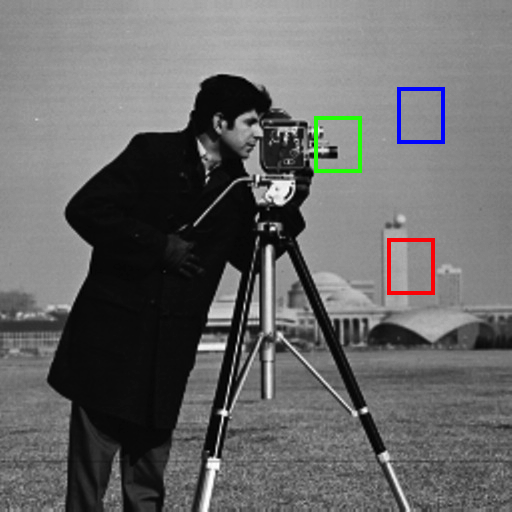
\includegraphics[width=0.5\linewidth]{fig/Input-test-images-a-Cameraman-grayscale-b-grayscale-Lena-and-c-color-Lena-All.png}
\caption{\label{fig:stereo_one} The three patches (windows) shown in the above figure does not contain the same amount of information. The blue patch is on an almost flat region, the red patch contains an edge and the green patch contains lots of edges, corners and flat regions.}
\end{figure}

Let us do the following exercise:

Your entry point for this part would be \cmd{evalSecondOrderStats}. You will be required to edit file \cmd{orderStatsHelper} for solutions to this part of the homework.
\begin{enumerate}
    \item \textbf{[3 points] Compute image derivatives}. Convert each image in the folder \cmd{../data/disparity} to gray scale images in function \cmd{gray} in file \cmd{orderStatHelper}. Once this is done, compute the image derivatives along $x$ and $y$ axes (the derivative along $x$ axis $I_x = I(x+h,y) - I(x,y)$, and similarly for y) in function \cmd{derivative}. \emph{You should be careful about the size of the image derivatives, as this would be important in the following steps}. As you might notice, this will result in images that contain edge information along a given direction. For this part your are not allowed to use OpenCV and ndimage libraries like image gradients or matlab functions like imgradient. You may read up on these and implement your own version to get the points for this question.
    
    \item \textbf{[9 points] Compute structure tensor map}. 
    Even though edge information of the objects present in an image might be useful in certain scenarios, some patches are more informative than others. Consider a patch on a blank textureless portion of the sky (the blue patch in Figure~\ref{fig:stereo_one}). This is not very useful for finding a matching patch between a stereo pair of images if we want to obtain depth from disparity.
   % often times patches like those marked in blue and red shown in Figure~\ref{fig:stereo_one} are not very informative and we need more information to understand specific object features. Thus we need to compute second order statistics. 
    To analyze the ``informativeness'' of an image patch, we wish to summarize the dominant directions of the edges present in that patch in terms of its second-order statistics. 
    For this we first compute the \emph{structure tensor map} (a structure tensor map is derived from the gradient of a function and summarizes predominant directions of gradients of the function in a specific neighborhood of a point). 
    \begin{enumerate}
        \item \textbf{[0 points]} Begin by specifying the window size for the given image.
        \item \textbf{[3 points]} Compute product of derivatives at every pixel by modifying function \cmd{product\_derivative}. You should remember that second order derivatives can be in direction $xx$, $yy$ and $xy$ (we treat $xy$ and $yx$ derivatives as commutative). 
        \item \textbf{[6 points]} For each pixel compute the sum of products of derivatives within the window around each pixel in function \cmd{sum\_of\_product\_derivatives}. The output for each pixel gives you the structure tensor map around each pixel. Specifically you should get the following matrix for each point $(u,v)$ in your image: 
        $M(u,v) = \begin{bmatrix}
            S_{xx}(u,v) & S_{xy}(u,v) \\
            S_{yx}(u,v) & S_{yy}(u,v)
        \end{bmatrix}$, 
        where $S_{xx}(u,v)$,  $S_{yy}(u,v)$ and $S_{xy}(u,v)$ are the sum of product derivatives around $(u,v)$.
    \end{enumerate} 
    \item \textbf{[3 points] Compute response at each pixel}. In function \cmd{det\_trace}, for each pixel $(u,v)$, compute
    \begin{enumerate}
        \item \textbf{[1 point]} the determinant of $M(u,v)$, and
        \item \textbf{[1 point]} the trace of $M(u,v)$.
        \item \textbf{[1 point]} For each point in the image compute $\frac{\texttt{determinant}}{\texttt{trace}}$ in function \cmd{inv\_harmonic\_mean}. This will generate a heat map which will be saved in the output folder.
    \end{enumerate}
    
 \item \textbf{[0 points] Postscript}.  The dominant directions of variance in the edges over a local neighborhood are captured by the eigenvalues of the structure tensor, $\lambda_1$ and $\lambda_2$. For a window over a flat region, both eigenvalues will be small. For a window over an edge, there will be one large eigenvalue due to the large gradient variation at the edge and a small eigenvalue associated with other minor gradients. But in a window containing a corner, both eigenvalues will be large \cite{forsyth2002computer}. Therefore, by comparing the two eigenvalues we can obtain information about the presence of edge and corner-like structures in an image patch.  The determinant of matrix $M$ computes the product of the eigenvalues of the matrix, while the trace computes the sum of eigenvalues. In other words, the ratio computed in part 3(c) is the inverse harmonic mean of the eigenvalues of $M$, which we can get without having to perform a time-consuming eigenvalue decomposition at each patch. 
 
In fact, it is this principle that is used to construct the Harris corner detection algorithm \cite{harris1988combined}. 

% The determinant of matrix $M$ computes the product of the eigenvalues of the matrix, while the trace computes the sum of eigenvalues. In other words the ratio computed in part 3.(c) is the inverse harmonic mean of the eigenvalues of $M$. 
%    %You might wonder why this is important. It is easy to show that response of M will vary along different positions in the image. 
% The dominant directions of variance in the edges over a local neighborhood are captured by the eigenvalues of the structure tensor, $\lambda_1$ and $\lambda_2$. We avoid the time-consuming eigenvalue computation by using  the trace and determinant of $M$.
%    For a window over a flat region, both the eigenvalues will be very small. For a window over an edge, one large eigenvalue associated at the edge and a small eigenvalue associated with other minor gradients. But in a corner window, both eigenvalues will be large \cite{}. In fact, it is this principle that is used to construct the Harris corner detection algorithm \cite{}. 
    
    \item \textbf{Deliverable}. Submit all the edits you made to file \cmd{orderStatsHelper}. Also attach the output of the final heatmap produced.
    
    
\end{enumerate}
\end{comment}
\section{Report Writing and Presentation [10 points]}

Please follow the guidelines for writing a good report.
Graders will penalize reports that are poorly written and fail to present the results in a reasonable manner.



\section{Extensions [10 points]}
Implement at least one of the following to get up to 10 points. You can implement multiple for extra credit!

\begin{itemize}
\item \textbf{Transformed color spaces for demosaicing.} Try your demosaicing algorithms by first interpolating the green channel and then transforming the red and blue channels R $\leftarrow$ R/G and B $\leftarrow$ B/G, i.e., dividing by the green channel and then transforming them back after interpolation. Try other transformations such as logarithm of the ratio, etc (note: you have to apply the appropriate inverse transform). Does this result in better images measured in terms of the mean error? Why is this a good/bad idea? 

\item \textbf{Evaluate alternative sampling patterns.} Come up with a way of finding the optimal 2x2 pattern for color sampling. You can further simplify this problem by fixing the interpolation algorithm to linear and only using non-panchromatic cells (i.e, no white cells). A brute-force approach is to simply enumerate all the $3^4 = 81$ possible patterns and evaluate the error on a set of images and pick the best. What patterns work well? What are their properties (e.g., ratio of red, blue, green, cells)?

\end{itemize}

%\bibliography{refs}
%\bibliographystyle{plain}
\end{document}